\chapter{Analisis}\label{chap:Analisis}
En el capítulo anterior se listaron distintas tecnologías que podían sernos útiles para nuestro proyecto. En el actual nos detendremos a explicar cuáles de ellas explicaremos y el por qué de su elección.

\section{Simulador de redes: GNS3}
Se ha decidido que GNS3 sea el simulador de redes a utilizar para nuestro proyecto por varias razones:
\begin{itemize}
\item Es \textbf{multiplataforma}, con lo que podemos trabajar sencillamente con él tanto desde Windows como Linux.
\item Existe \textbf{mucha información} para consultar. Desde internet contamos con documentación oficial y un foro propio. Hay incluso libros sobre él y como ejemplo tenemos el usado en varias ocasiones en este documento, ``The Book of GNS3'', por Jason C. Neumann.
\item Es altamente \textbf{expandible}: hay decenas de aparatos reales que pueden incluirse y emularse en las topologías creadas. Pueden descargarse desde \MYhref{https://www.gns3.com/marketplace/appliances}{su marketplace}.
\item \textbf{Cuenta con una API REST} que lo hace interactivo desde el exterior.
\end{itemize}

GNS3 se estructura en \textbf{proyectos}. En cada proyecto podemos desplegar una serie de dispositivos y conectarlos entre sí. Al guardar un proyecto como tal, el despliegue realizado se guarda junto a él. Sin embargo, el estado de las máquinas no corre la misma suerte, y es que a cada apagado de las mismas toda su configuración se pierde.

Una de las características más interesantes de GNS3 y sus proyectos está en la importación y exportación de estos. El simulador cuenta con una opción que permite extraer todo un proyecto en una imagen (de formato \textit{.gns3project} para que sea fácilmente portable. Existe la posibilidad de exportar, junto a la topología creada, las imágenes base sobre las que los nodos del proyecto están construidas para que no sea necesario contar con esas imágenes en GNS3 donde se pretende importar.

\begin{figure}[h]
  \centering
  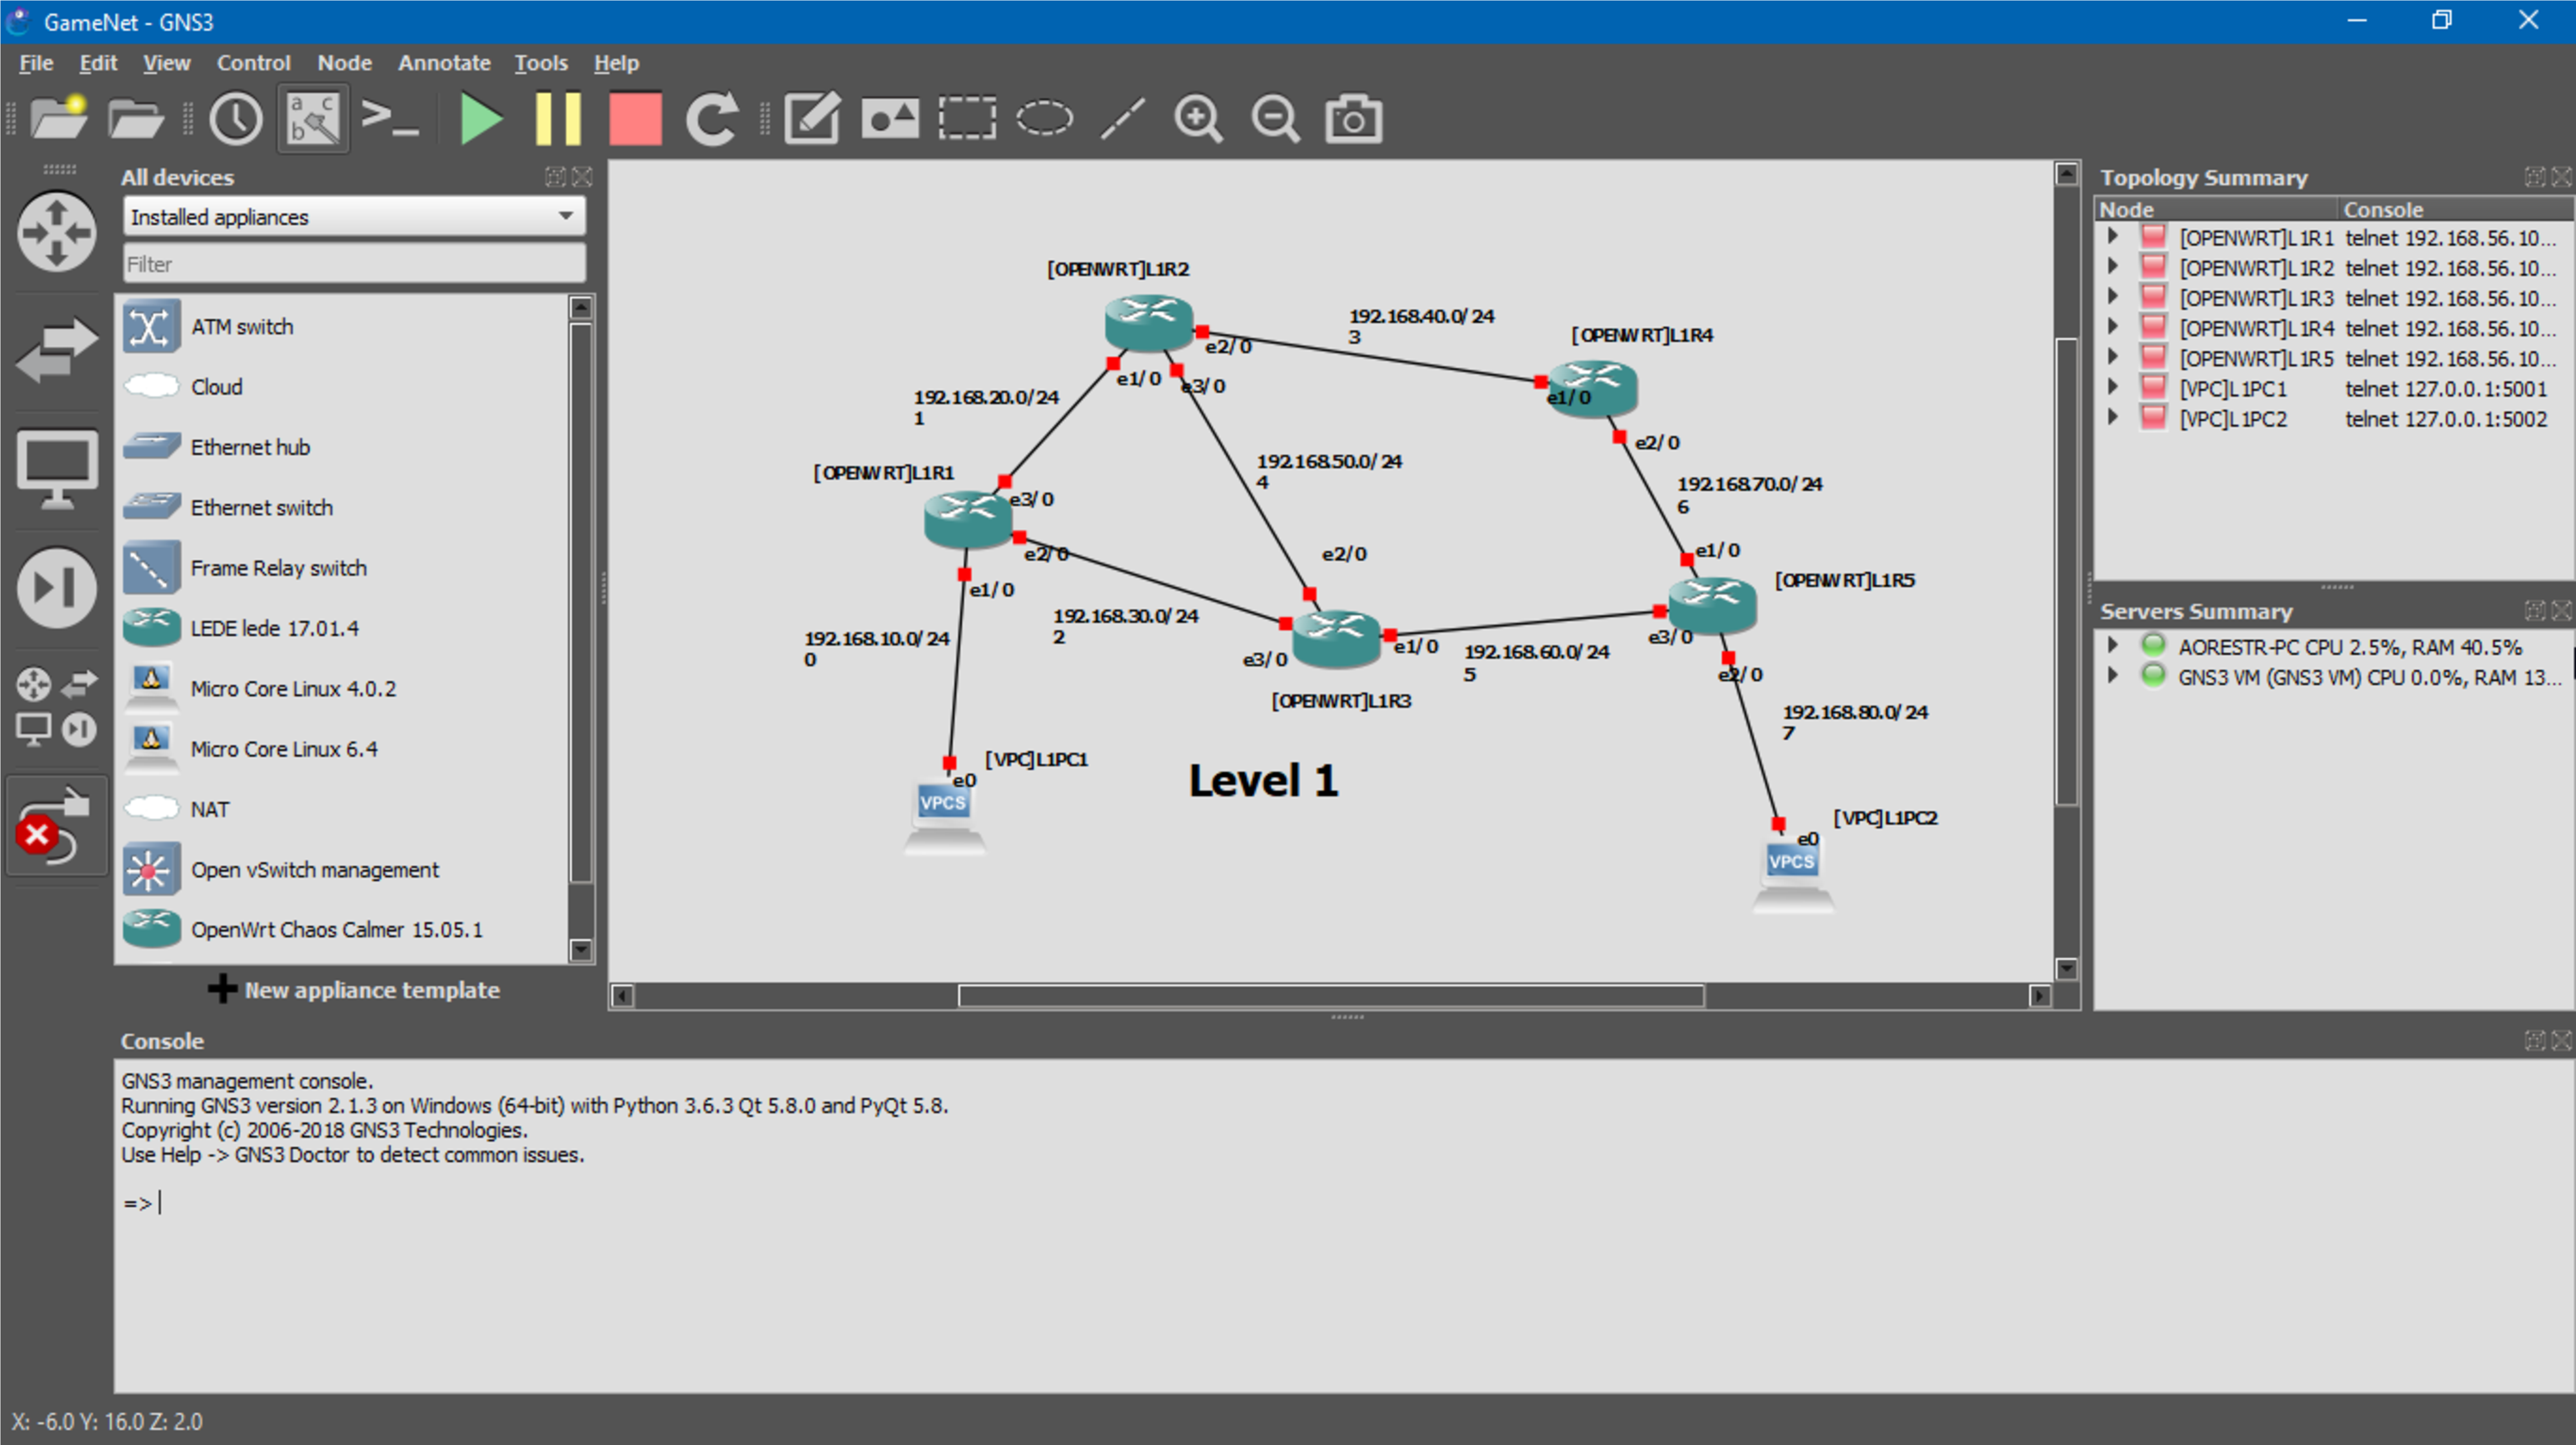
\includegraphics[scale=0.15]{imagenes/interfazgns}
  \caption{Interfaz de GNS3}
  \label{fig:interfazgns}
\end{figure}

La interfaz de usuario de la aplicación puede verse en la figura \ref{fig:interfazgns}. La barra de arriba está repleta de opciones relacionadas con el proyecto, como arrancar todos los dispositivos, pausarlos, pararlos o incluso herramientas de dibujo para convertir el esquema en algo más intuitivo y legible. A la izquierda se listan los nodos disponibles en la máquina. Arrastrándolos al centro los insertamos en el proyecto.

A continuación pasaremos a explicar conceptos clave del emulador.

\subsection{El servidor}

\subsubsection{La API}
Una API (que será explicada más adelante)
La primera vez que aparezca un acrónimo, debes indicar cuál es su significado. De hecho, en los títulos o como primera palabra de la frase, (o en el abstract) hay que evitar las abreviaturas.

\subsubsection{Nodos}
Cada elemento de una red está representado en GNS3 por un elemento llamado \textbf{nodo}. Estos nodos, que pueden ser desde un router a un switch, no son más que virtualizaciones de aparatos reales. Por norma general, estas virtualizaciones se realizan a partir de imágenes de los sistemas operativos que se integran en los aparatos. Así, podemos tener varios routers distintos de Cisco montados sobre la misma estructura, permitiéndonos jugar con ellos con verdadera facilidad.

GNS3 es usado ampliamente como método de entrenamiento para los exámenes de Cisco. Tal es así, que en su academia se pueden encontrar cursos para facilitar la \MYhref{https://academy.gns3.com/p/the-complete-networking-fundamentals-course-your-ccna-start/?product_id=169831&coupon_code=HOMEPAGE}{obtención del CCNA}. Sin embargo, las imágenes de las máquinas de Cisco, aunque pueden ser encontradas fácilmente en internet, requieren de licencia para ser usadas. Siendo así se optó por hacer uso de software libre para el proyecto.

\subsubsection{Enlaces}

\section{Motor de videojuegos: Unity}
realmente esta elección no era tan complicada